\pdfminorversion=4
\pdfobjcompresslevel=0
\documentclass[iicol,pdflatex,sn-mathphys-num]{sn-jnl}
\usepackage[T1]{fontenc}
\usepackage{graphicx,booktabs,tabularx,array,amsmath,amssymb}
\usepackage{enumitem,xurl,placeins,microtype}
\raggedbottom
\setlength{\emergencystretch}{2em}
\setlist{nosep,leftmargin=*}
\graphicspath{{../../data/scored/proquest/paper_low_cost_v1/}{../../data/scored/proquest/paper_jcss_v1/}}
\newcommand{\note}[1]{\par\vspace{3pt}{\footnotesize\textit{Notes:} #1\par}}
\newcommand{\evidence}[1]{\textsuperscript{\hyperref[app:evidence]{[#1]}}}
\newcommand{\pathcode}[1]{{\footnotesize\path{#1}}}
\begin{document}
\title[Validating newspaper economic forecasts]{From newspaper text to economic forecasts: Human validation and measurement sensitivity}
% Author details must be confirmed before submission; no affiliations are inferred.
\author*{\fnm{Bode} \sur{Bosell}}\email{bodeb@bu.edu}
\abstract{Newspaper archives record economic expectations, but extracting a forecast and defining its evaluable meaning are distinct measurement tasks. We study 365,188 retained forecast candidates from selected United States newspapers spanning 1900--2026, of which 232,741 satisfy deterministic scoring and outcome-availability rules. Two human reviewers assess the same 300 source-linked candidates, agreeing on inclusion decisions in 91.7\% of cases while each rejecting more than one-quarter of the sample. In this combined, unweighted audit, a single additional GPT-4o mini verification pass raises inclusion precision from 70.7--71.0\% to 77.0--77.4\% against the first reviewer and from 68.0\% to 75.9\% against the second, while removing 14 and 9 human-accepted claims, respectively. Agreement on specific annotations shows little consistent improvement, distinguishing candidate filtering from reliable interpretation. On a matched subset of 9,260 employment claims, measured accuracy ranges from 34.2\% to 57.6\% across outcome bands, and replacing unemployment with payroll employment reverses the baseline-relative point estimate. Predictive applications remain exploratory and do not establish stable incremental skill. The contribution is an auditable measurement analysis showing that improved candidate precision does not establish more reliable forecast interpretation or a robust economic performance conclusion.}
\keywords{computational social science, economic expectations, newspaper archives, language models, measurement validity, forecast evaluation}
\maketitle

\section{Introduction}
Newspapers preserve expectations expressed outside formal forecasting surveys. A business leader may anticipate recovery, an economist may expect unemployment to rise, and an editorial may predict lower prices. These statements are useful evidence about beliefs at a particular time. Making them comparable observations requires identifying who predicts what, for which economy, and over what horizon. A forecast of slowing growth differs from a forecast of falling output; an employment forecast need not concern the unemployment rate.

Language models can generate structured candidates from such archives at scale. The social-science question is whether the resulting measurements support the interpretation assigned to them. An inclusion filter can remove passages that are not forecasts while leaving errors in the targets and horizons of the remaining passages. A numerical outcome can then be attached consistently to a misinterpreted claim. We study this sequence directly, separating candidate validity, annotation agreement, and economic evaluation.

The primary corpus contains 274,070 machine-verified ProQuest candidates from annual exports for 1900--2010; 175,855 satisfy the inherited deterministic scoring rules. A separate modern extension covers 2011--2026, with 91,118 retained candidates and 56,886 mature, supported claims evaluated. The economic analyses report historical and modern estimates separately because their retrieval, review, and outcome-availability conditions differ.

The first contribution is a paired source-validation analysis. Two human reviewers evaluate the same 300 candidates, with source lineage and prior machine-label exposure documented. Their historical inclusion decisions agree on 233 of 250 claims, but the reviewers accept only 177 and 171, respectively. Agreement between humans therefore does not imply that the original automated candidate set has high precision. The two reviews remain separate references rather than an adjudicated gold standard.

The second contribution is a completed additional-pass experiment on that exact reviewed sample. One further GPT-4o mini verification attempt per claim removes 43 candidates. Historical inclusion precision increases by approximately 6.8 and 8.2 percentage points against the two reviewers, but some human-accepted claims are also removed. The retained claims keep their original annotations. Agreement on those annotations improves little and sometimes declines: exact historical horizon agreement falls for both reviewers. This identifies an empirical limit of repeated inclusion filtering as a remedy for measurement error.

The third contribution is an economic sensitivity analysis on fixed observations. Among 9,260 matched historical employment claims, measured accuracy rises from 34.2\% under the original unemployment band to 57.6\% under sign-only scoring. The simple comparison forecast improves even more, so the relative advantage shrinks. Replacing falling unemployment with rising payroll employment changes the baseline-relative point estimate from positive to negative. These results demonstrate that a favorable hit rate cannot identify a defensible interpretation of what the source predicted.

The contribution is application-specific evidence about the consequences of measurement choices, rather than a new extraction architecture or a universal ranking of language models. Historical forecast interpretation, news-based economic indicators, and automated text validation all have direct predecessors. Our paired audit connects these questions in one source-linked application: improved candidate selection leaves substantial interpretation problems, and economically reasonable outcome mappings lead to different comparative conclusions.

Predictive applications are secondary checks. Frozen claim models transfer to the modern extension with uneven calibration and a pronounced employment failure. A historical monthly experiment finds a small average gain from newspaper features, but its interval includes zero and the sign reverses when the already-inspected 2007--2009 evaluation months are omitted. The paper can therefore inform the construction of expectations data without claiming stable forecasting superiority.

\section{Related research and the scope of the contribution}
\subsection{Historical expectations, sentiment, and uncertainty}
Historical forecast interpretation has direct precedents. \citet{mathy2017} quantify contemporaneous and forward-looking assessments in the business press during the Great Depression. Their object is close to ours: what economic observers believed while events unfolded. Our longer annual corpus and automated candidate generation extend the scale of this inquiry; they do not originate the use of historical press statements to study expectations. The contribution here is a documented chain from extraction choices to claim interpretation and baseline-relative outcomes.

The broader text-as-data literature provides the statistical setting \citep{gentzkow2019}. Newspaper-derived constructs need not be explicit forecasts. \citet{bybee2024} extract topical attention from business news and examine its relationship with economic activity, including incremental information beyond conventional indicators. \citet{barbaglia2022} use aspect-specific news sentiment for macroeconomic forecasting. These approaches motivate a demanding comparison with macro-only predictors, but their targets differ from the correctness of an attributable statement. A topic can be informative without containing a forecast; an explicit forecast can be incorrect while revealing a valuable historical belief. No common-data replication against those published signals is attempted here.

Financial-news research supplies another relevant distinction. \citet{tetlock2007} links pessimistic language in a Wall Street Journal column to market behavior. \citet{garcia2013} studies news sentiment and stock-return predictability, finding that the predictive relationship is concentrated in recessions. These studies establish substantive precedents for extracting economically informative language. They do not imply that every negative sentence predicts a price decline, or that a sentiment coefficient measures a newspaper forecaster's accuracy. For our application, the relevant comparison must align the quoted proposition, asset or macroeconomic target, forecast origin, and horizon. A sentiment index and a directional claim may contain related information without being interchangeable measurements.

\citet{baker2016} develop newspaper-based measures of economic policy uncertainty and validate their construction using several forms of evidence, including human readings. Their historical US index reaches back to 1900 \citep{bakerhistorical}. It offers a natural comparison for a long-run newspaper corpus, but measures policy-related uncertainty rather than the correctness of particular forecasts. The documented historical index also uses source-specific normalization and overlapping newspaper sets. That design highlights a limitation of our exports: without a complete article-processing denominator, raw forecast counts cannot be interpreted as a coverage-normalized attention index. We do not estimate a relationship with EPU in this paper; adding its series to a future comparison would require a documented alignment and an explicit account of changing source coverage.

\subsection{Professional forecasts and the meaning of confidence}
The Livingston Survey \citep{philalivingston} and Survey of Professional Forecasters (SPF; \citealp{philaspf}) supply established records of explicitly elicited economic expectations. The former began in 1946 and the latter in 1968. Federal Reserve staff projections are separately available in the Philadelphia Fed's Tealbook/Greenbook datasets \citep{philagreenbook}. These records are potential external comparators, rather than observations included in the newspaper sample or benchmarks already tested here. A valid comparison would harmonize the economic variable, units, target period, release vintage, and information date before evaluating relative performance. Survey response dates, newspaper publication dates, and staff forecast dates need not describe identical information sets. In particular, the staff projections become public only after a five-year lag; their historical forecast date alone does not make their contents an admissible contemporary public predictor.

\citet{campbell2024} examine probabilistic SPF forecasts and find evidence of overprecision, with little evidence of optimistic bias. Their analysis distinguishes confidence in outcomes from the direction of forecast errors and uses an exploration--validation design. This distinction matters for our interpretation of linguistic confidence. An extracted label such as confident or hedged is not an elicited probability distribution. A low directional hit rate therefore does not, by itself, demonstrate overprecision, and confident language cannot be assigned a numerical probability without a separately validated mapping. Conversely, the probability produced by our claim-correctness model concerns whether a machine-scored label will be correct; it is not the probability originally expressed by a historical speaker. We make no claim to reproduce the SPF overprecision result with newspaper labels.

\subsection{Text measurement and extraction validation}
Validation must match the intended construct. \citet{shapiro2020} compare sentiment measures with human ratings and separately investigate economic applications. \citet{grimmer2013} emphasize problem-specific validation of automated text analysis. \citet{loughran2011} demonstrate that general-purpose negative-word lists can misclassify language in financial filings, motivating domain-specific measurement. Their evidence concerns dictionaries and 10-Ks, not our newspaper extractor; its relevance is the need to validate the interpretation assigned to language in its own setting. For the present study, agreement about the text and success at predicting an economic series are separate requirements. A model's association with future production cannot substitute for checking that the source actually made the forecast attributed to it.

Low-cost language-model annotation is itself established research. \citet{gilardi2023} compare ChatGPT classifications with human annotations across several text tasks and document cost advantages in those applications. Our ProQuest review evaluates inclusion and economic annotations in newspaper forecasts; it does not establish a model ranking that transfers across domains. The contribution is therefore application-specific evidence, including adverse results, rather than a claim that inexpensive automated annotation is newly possible.

\subsection{Forecast evaluation, revisions, and model selection}
Proper scoring rules provide a foundation for evaluating probabilistic forecasts \citep{gneiting2007}. Brier loss and log loss assess probabilities, whereas directional accuracy evaluates categorical decisions and AUC evaluates ranking. These measures answer different questions. A proper probability score cannot repair an incorrectly defined outcome: the economic target must first correspond to the proposition being evaluated. Likewise, differences in target prevalence make scores from different samples unsuitable as direct measures of a model's improvement. Our comparisons therefore emphasize matched observations, explicit targets, and the same baseline predictions under each stated rule.

Historical prediction also requires careful treatment of data revisions. \citet{croushore1999} explain how real-time vintages differ from later datasets. We distinguish print-time predictor information, labels admitted to model fitting, and revised outcomes used for retrospective assessment. The selected historical macro benchmark reconstructs vintage information for fitting; the claim-correctness exercise uses frozen revised assessment series and a release allowance. These are different evidentiary standards, and we do not describe the latter as a complete recreation of historical real-time forecasting.

Finally, \citet{cawley2010} show how optimization of a finite-sample model-selection criterion can introduce selection bias in reported performance. Chronological separation addresses information ordering, but cannot restore an untouched evaluation sample after its results have influenced analysis choices. This motivates our disclosure of prior outcome exposure and the exploratory status of the saved extension. 

\section{Data, lineage, and the extraction workflow}
\subsection{Historical corpus and analysis population}
The historical newspaper source is ProQuest \citep{proquesthistorical}, with source access and text analysis organized through its TDM Studio environment \citep{proquesttdm}. The received exports, rather than a provider product description, define the actual analysis population. The source consists of 111 annual raw shards and 111 annual machine-verified shards spanning 1900--2010. The archived exports were copied unchanged from the integration repository at commit \texttt{774b68f}. The raw files contain 488,660 candidate claims; the verified files contain 274,070. The latter represent 146,720 article identifiers, including 105,604 articles with at least one retained claim and 41,116 articles represented only by a no-prediction record. These article counts describe the received exports, not the universe of newspaper articles searched or processed.\evidence{H1}

Table~\ref{tab:flow} summarizes the historical analysis population and scoring exclusions. The newspaper families include the New York Times, Wall Street Journal, Los Angeles Times, Chicago Tribune, Washington Post, Boston Globe, Barron's, and Christian Science Monitor, with a small USA Today component. Historical edition labels are consolidated for descriptive paper-family comparisons. Coverage is uneven: verified Wall Street Journal claims begin in 1984, and scored Chicago Tribune coverage ends in 2001. Consequently, differences over time or across publishers can reflect changes in source composition. The corpus should be described as forecasts reported in selected newspapers, not a probability sample of the American press.

\begin{table*}[t]
\caption{Historical corpus and deterministic-scoring flow}\label{tab:flow}
\centering\small
\begin{tabularx}{\linewidth}{Xr}
\toprule
Stage or mutually exclusive exclusion & Claims / records\\
\midrule
Raw annual candidate claims & 488,660\\
Machine-verified candidate claims & 274,070\\
\quad Not explicitly US-national & 80,183\\
\quad Topic without a defensible benchmark & 7,894\\
\quad No scorable direction & 3,176\\
\quad Numeric horizon outside 1--24 months & 2,490\\
\quad Outside benchmark coverage & 2,297\\
\quad Unusable horizon label & 2,175\\
\midrule
Scored under the inherited historical rules & 175,855\\
\quad Of which: pre-1919 business claims using an NBER proxy & 1,047\\
Eligible for the claim-correctness model before split purging & 174,808\\
\bottomrule
\end{tabularx}
\note{The six exclusion rows sum to 98,215; 274,070 minus 98,215 equals 175,855. The NBER-proxy row is a subset of scored claims, not another descriptive exclusion. The 41,116 no-prediction export records are not candidate claims. Raw and verified exports are not a fully reconciled processing ledger; their difference is not labeled a measured rejection count. Sources: H1--H2 and P2, Appendix~\ref{app:evidence}.}
\end{table*}

Machine verification is an inclusion filter. It is not independent human validation. The inventory contains 696 verified rows with identical exported labels; all are retained. Because the local exports omit quotations and lack a unique claim identifier, distinct passages can share the same categorical labels. Deduplication on those fields alone would impose an unsupported assumption about identity. We instead preserve file, line, publication date, and article linkage.\evidence{H1}

\subsection{Modern extension and evaluation population}
The separate 2011--2026 export contains 91,118 retained candidates. Excluding 19 default-kept verification exceptions leaves 91,099 primary inputs; 33,071 no-prediction records are kept outside the candidate count. Eligibility and maturity rules remove 32,604 unsupported claims, 1,138 claims with unmatured outcomes, and 471 with reference gaps, leaving 56,886 evaluated claims from 23,775 articles. These are saved October 20, 2026 results, with no interpolation of unavailable outcomes. The historical and modern populations are reported separately in the methods and results.\evidence{N1}

Human source review includes 50 modern candidates sampled across all sixteen publication years. That sample assesses extraction and annotation, including candidates without mature economic outcomes; it is not a random subsample of only the 56,886 evaluated claims. The modern predictive exercise applies frozen historical claim models, but undocumented prior outcome exposure prevents describing it as an untouched confirmatory holdout. Appendix~\ref{app:modern} records the dated reference coverage and model comparisons.

\subsection{From article text to an evaluable claim}
Figure~\ref{fig:pipeline} summarizes the workflow. The workflow has five steps. Article text is retrieved within the authorized source environment. An extractor proposes forecast spans and structured labels. A verifier evaluates candidates. Permitted categorical information is exported with source-linked addresses, while the original exports are preserved. Finally, explicit eligibility and outcome-availability rules determine which claims enter each analysis. The historical human comparisons identify the original ProQuest labels as GPT-4o mini outputs \citep{openai4omini}.\evidence{V1--V2}

\begin{figure*}[t]
\centering
\setlength{\fboxsep}{7pt}
\fbox{\begin{minipage}{.92\linewidth}\small
\textbf{Authorized article text}\hfill Source access and publication date\\[4pt]
$\downarrow$\quad Candidate extraction: passage, topic, direction, horizon, scope, attribution\\[4pt]
$\downarrow$\quad Machine verification: retain or reject proposed candidates\\[4pt]
$\downarrow$\quad Frozen categorical export: preserve article and source-row lineage\\[4pt]
$\downarrow$\quad Source review and explicit analysis-eligibility rules\\[4pt]
\textbf{Two distinct outputs:} textual validity and field agreement; economic outcomes under a stated scoring rule
\end{minipage}}
\caption{A workflow with separate textual and economic checks. Human review evaluates sampled candidates; it does not certify every exported row.}
\label{fig:pipeline}
\end{figure*}

Language models were used as measurement instruments for candidate extraction and verification. The new audit pass is documented in the validation section, including the returned snapshot and failure policy. AI assistance was also used to organize code, calculate comparisons, and draft and revise this manuscript. Human reviewers supplied the source judgments; their labels were not generated by the additional verifier. The authors must review and take responsibility for the analysis and final text before submission.

The main fields are topic, economic direction, horizon, geographic scope, confidence language, voice, speaker, and current conditions. They serve different purposes. Topic selects a potential outcome series. Scope prevents a regional or foreign forecast from being judged against a national US aggregate. Horizon determines the endpoint. Attribution separates a newspaper's own assessment from a forecast it reports. Confidence describes language and is not a calibrated probability. Present conditions must be distinguished from a prediction even when both appear in the same paragraph.

The inclusion rubric requires a falsifiable claim about future economic conditions. It excludes current or retrospective descriptions, advertisements, generic rules, non-economic promises, and hypothetical scenarios without a committed forecast. Reporting a forecast skeptically does not necessarily erase the forecast, but republishing one after its outcome is known creates a timing problem. These boundaries matter because a hindsight description scored as a forecast can manufacture apparent predictive skill. Source context, rather than categorical labels alone, resolves such cases.

\subsection{What the received data cannot establish}
The local exports do not supply complete article-processing denominators. A rise in claim counts therefore cannot be interpreted directly as greater attention to the economy. It may reflect retrieval coverage, article availability, extraction yield, or verification behavior. Likewise, fewer verified than raw claims do not identify the number of genuine forecasts removed. The raw set is a sensitivity sample under the same scoring rules, not a second human reference standard.

The pipeline preserves retrospective window annotations and verifier prose outside model inputs. Neither is available as an admissible print-time predictor. All reported historical economic estimates use the annual ProQuest exports and exclude old crisis-window exports.

\section{Human validation and an additional verification pass}
\subsection{Sampling, source linkage, and reviewer exposure}
Two human reviewers evaluated the same 300 claims from 299 distinct articles: 250 historical and 50 modern. The first review was confirmed by the author as human work without AI assistance; the second review's frozen labels and author attestation are preserved separately. Reviewer 2 read source passages and context without consulting claim-level machine labels, the first reviewer's decisions, or realized outcomes. Aggregate study summaries had been visible. The first review had mixed machine-label exposure, so the design is not described as fully blinded.\evidence{V1--V4}

The original historical batch contains 150 claims from a frame of 175,843 scored verified candidates after excluding 12 pilot records. It retains an initial simple random sample of 100 and adds 50 without replacement. The initial 100 had prior machine-label exposure; the added 50 had machine labels hidden until annotation was frozen. A further historical batch samples 100 without replacement from the 175,693 remaining eligible addresses. All sampled sources were recovered and matched to the saved export addresses.

The modern batch is stratified by publication year: four records from each of 2011 and 2026 and three from each intervening year. Its frame contains 91,118 retained candidates, including verification exceptions omitted from the predictive analysis. Modern candidates need not have mature or scorable outcomes. We report unweighted descriptive audit proportions by frame; they are not population-weighted modern estimates. Pooling the 300 observations would combine different eligibility and sampling designs.

\subsection{Inclusion decisions and human agreement}
Table~\ref{tab:review} reports both reviewers' decisions. Historical agreement is 233/250 (93.2\%); among the 249 cases resolved by both reviewers, it is 233/249 (93.6\%). Historical Cohen's kappa is 0.840 when unclear is retained as a third category and 0.847 on resolved cases. Modern agreement is 42/50 (84.0\%). Across both frames, 196 claims are included by both reviewers, 79 excluded by both, and 25 have different decisions, including one unclear decision. These counts preserve disagreement rather than replacing it with a consensus label.\evidence{V4}

\begin{table*}[t]
\caption{Two-reviewer inclusion decisions on the same source-linked candidates}\label{tab:review}
\centering\small
\begin{tabularx}{\linewidth}{Xlrrrr}
\toprule
Frame & Reference & Reviewed & Include & Exclude & Unclear\\
\midrule
Historical & Reviewer 1 & 250 & 177 & 72 & 1\\
Historical & Reviewer 2 & 250 & 171 & 79 & 0\\
Modern & Reviewer 1 & 50 & 35 & 15 & 0\\
Modern & Reviewer 2 & 50 & 33 & 17 & 0\\
\bottomrule
\end{tabularx}
\note{These are candidate-audit counts, not economic correctness or full-document recall. The historical sample is drawn from scored verified candidates; modern sampling covers retained candidates by year. Reviewer judgments remain separate. Source: V4.}
\end{table*}

\subsection{A single additional pass on the reviewed sample}
All 300 sampled candidates had explicitly passed the saved production verifier. We therefore evaluate a further filter on survivors, not the effect of the original production verification step. On October 22, 2026, GPT-4o mini was called once for each sampled claim inside the authorized ProQuest environment, using the existing verifier prompt, the candidate quotation, source context, publisher, and date. Neither human decisions nor prior verdicts, verifier explanations, or economic outcomes entered the prompt. Each request used temperature zero and a maximum of 256 output tokens; retries were disabled. All responses reported model snapshot \texttt{gpt-4o-mini-2024-07-18}. Prepared-request hashes and per-claim attempt records preserve the run specification.\evidence{V5}

The 300 attempts returned 256 valid keep decisions, 43 valid drop decisions, and one response that failed strict verdict parsing. The unresolved response was not retried and is conservatively retained, leaving 257 candidates: 214 historical and 43 modern. Human judgments were frozen before this run. The experiment changes only inclusion; it performs no new extraction and revises no original annotation.

For reviewer $r$, let $H_{ir}=1$ denote an accepted candidate and $K_i=1$ denote retention by the additional filter. Sample precision before and after filtering is
\begin{equation}
 P_r=\frac{\sum_i H_{ir}}{n},\qquad
 P'_r=\frac{\sum_i K_iH_{ir}}{\sum_i K_i}.
\end{equation}
The unclear human case is assigned zero and one to form bounds, using the same assignment before and after. These bounds express unresolved annotation, not sampling confidence intervals. Retention of human-accepted candidates is $\sum_i K_iH_{ir}/\sum_i H_{ir}$; it is not recall over all forecasts in the newspaper sources.

\begin{table*}[t]
\caption{Inclusion precision after one additional verification pass}\label{tab:reverify}
\centering\small
\begin{tabularx}{\linewidth}{Xlrrrrr}
\toprule
Frame & Reference & Before (\%) & After (\%) & Change (pp) & Invalid removed & Valid lost\\
\midrule
Historical & Reviewer 1 & 70.8--71.2 & 77.6--78.0 & +6.77--6.84 & 25 & 11\\
Historical & Reviewer 2 & 68.4 & 76.6 & +8.24 & 29 & 7\\
Modern & Reviewer 1 & 70.0 & 74.4 & +4.42 & 4 & 3\\
Modern & Reviewer 2 & 66.0 & 72.1 & +6.09 & 5 & 2\\
\bottomrule
\end{tabularx}
\note{Historical denominators fall from 250 to 214; modern denominators from 50 to 43. The one unresolved model response is retained. Ranges concern the single unclear human decision. ``Invalid'' and ``valid'' are relative to the named reviewer, not adjudicated truth. These are descriptive paired sample changes without a population-weighted estimate or a significance claim. Source: V5.}
\end{table*}

Table~\ref{tab:reverify} reports inclusion precision and accepted-claim losses. The historical filter retains 166/177 (93.8\%) of Reviewer 1's accepted claims and 164/171 (95.9\%) of Reviewer 2's. Modern retention is 32/35 (91.4\%) and 31/33 (93.9\%). The gain in inclusion precision therefore comes with loss of accepted material. The original production pass's precision gain remains unidentified by this sample because candidates it rejected were not reviewed.

\subsection{Specific labels before and after filtering}
Figure~\ref{fig:human} contrasts inclusion precision with direction and horizon agreement. Field agreement compares original machine annotations with each reviewer's labels, conditional on that reviewer accepting the claim. It has a different denominator from inclusion precision. Table~\ref{tab:fields} reports all eleven fields for the historical sample; Appendix~\ref{app:labels} reports the modern fields and summarizes human--human agreement. Missing or explicitly uncertain fields receive no match credit. Literal not-applicable matches remain included. Category-level precision, recall, support, and confusion counts are retained in the reproducibility files and use only resolved comparable fields.\evidence{V4--V5}

\begin{table*}[t]
\caption{Historical machine--human label agreement before and after filtering}\label{tab:fields}
\centering\small
\begin{tabularx}{\linewidth}{Xrrrr}
\toprule
& \multicolumn{2}{c}{Reviewer 1} & \multicolumn{2}{c}{Reviewer 2}\\
Field & Before & After & Before & After\\
\midrule
Topic & 156/177 (88.1\%) & 148/166 (89.2\%) & 152/171 (88.9\%) & 146/164 (89.0\%)\\
Direction & 154/177 (87.0\%) & 145/166 (87.3\%) & 148/171 (86.5\%) & 143/164 (87.2\%)\\
Price direction & 132/177 (74.6\%) & 125/166 (75.3\%) & 127/171 (74.3\%) & 123/164 (75.0\%)\\
Unemployment direction & 150/177 (84.7\%) & 140/166 (84.3\%) & 145/171 (84.8\%) & 139/164 (84.8\%)\\
Horizon (months) & 115/177 (65.0\%) & 106/166 (63.9\%) & 118/171 (69.0\%) & 112/164 (68.3\%)\\
Confidence & 130/177 (73.4\%) & 124/166 (74.7\%) & 127/171 (74.3\%) & 121/164 (73.8\%)\\
Voice & 136/177 (76.8\%) & 126/166 (75.9\%) & 127/171 (74.3\%) & 121/164 (73.8\%)\\
Speaker name & 117/177 (66.1\%) & 107/166 (64.5\%) & 101/171 (59.1\%) & 96/164 (58.5\%)\\
Scope & 114/177 (64.4\%) & 108/166 (65.1\%) & 113/171 (66.1\%) & 108/164 (65.9\%)\\
Quoted forecaster & 131/177 (74.0\%) & 122/166 (73.5\%) & 129/171 (75.4\%) & 123/164 (75.0\%)\\
Current state & 55/72 (76.4\%) & 53/70 (75.7\%) & 123/171 (71.9\%) & 120/164 (73.2\%)\\
\bottomrule
\end{tabularx}
\note{Exact agreement on each reviewer\textquotesingle s included claims. Different before/after denominators reflect filtering, not relabeling. Reviewer 1 current-state comparisons omit the original historical batch because its coding convention differs. NA matches are included; missing/uncertain fields receive no match credit. Source: V5.}
\end{table*}

Historical topic and direction agreement remain relatively high, while horizon and scope are weaker. The filter changes exact horizon agreement from 115/177 (65.0\%) to 106/166 (63.9\%) against Reviewer 1 and from 118/171 (69.0\%) to 112/164 (68.3\%) against Reviewer 2. Historical scope agreement rises by 0.7 percentage points for Reviewer 1 but falls by 0.2 points for Reviewer 2. These small, mixed changes do not support interpreting repeated filtering as annotation repair. On identical retained claims, label agreement is unchanged by construction.

\begin{figure*}[t]
\centering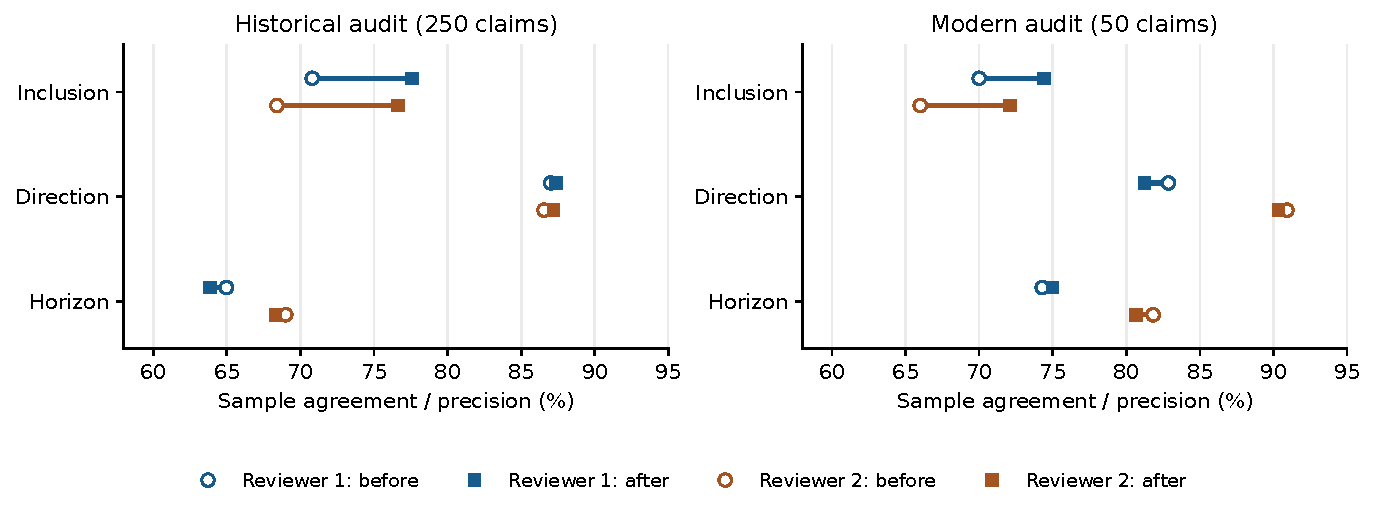
\includegraphics[width=\linewidth]{validation_stages.pdf}
\caption{Inclusion precision and annotation agreement answer different questions. Each point is a descriptive sample percentage against one human reviewer. Inclusion is measured on all sampled candidates; direction and horizon agreement are conditional on that reviewer's inclusion. Historical and modern frames remain separate. Bars connecting before and after values indicate filtering-induced changes, not revised annotations. Reviewer 1 inclusion uses the lower bound for the unclear historical case}\label{fig:human}
\end{figure*}

Some apparent label disagreements concern conventions rather than incompatible meanings. Horizon coding maps approximately four to eight months to six and nine to fifteen months to twelve; agreement does not establish an exact source endpoint. Speaker names are compared literally, so abbreviations can disagree while identifying the same person. Price and unemployment agreement contains not-applicable matches and cannot be read as accuracy among only substantive price or unemployment forecasts. The original first-review current-state convention differs from the later convention; those comparisons are omitted rather than combined into a misleading all-fields score.

\subsection{What the validation supports}
Inclusion, field agreement, document-level recall, and economic correctness are distinct quantities. The human audit evaluates the first two, and the extra pass demonstrates their different responses to filtering. Neither exercise measures forecasts that candidate extraction omitted. Nor does agreement on a coarse horizon or topic establish that the economic scoring endpoint matches the source proposition.

The review identifies present or past descriptions treated as forecasts, unresolved conditionals, ambiguous attribution, coarse horizons, and scope mismatches. The local categorical records do not contain a consistent frequency table for these error explanations, so we do not invent one. For example, slower inflation need not mean falling prices, and stronger job growth need not mean falling unemployment.

The historical outcome analyses that follow use the original machine-selected, machine-labeled corpus. We do not refit those analyses on the selectively retained audit subset or multiply full-corpus accuracy by an inclusion fraction. Such adjustments would require an explicit estimand, sampling weights, and assumptions about how interpretation errors relate to topic, era, horizon, and realized outcomes.

\section{Measurement choices and historical forecast evaluation}
\subsection{The scoring contract}
For claim $i$, let $m_i$ denote its publication month, $h_i$ its assigned horizon, $q_i$ its target, and $d_i$ its normalized direction. A scoring specification $s$ maps the target and dates to an outcome $y_i^{(s)}$. Correctness is
\begin{equation}
 z_i^{(s)}=\mathbf{1}\{d_i=y_i^{(s)}\}.
 \label{eq:correct}
\end{equation}
This is a definition of correspondence under an interpretation, not a direct measurement of whether the historical speaker understood the economy. If $q_i$ or $h_i$ misrepresents the passage, $z_i^{(s)}$ can be computed exactly and still answer the wrong substantive question.

The inherited outcome rule compares the publication-month level with the level $h_i$ months later. For production, prices, and markets, the change is $100(X_{m_i+h_i}/X_{m_i}-1)$; for unemployment it is the difference in rate percentage points. The original flat bands are $\pm2\%$ for industrial production, $\pm5\%$ for the nominal Shiller S\&P Composite price series, $\pm1.5\%$ for CPI, and $\pm0.5$ percentage points for unemployment. Changes exactly at a boundary count as flat, subject to the saved numerical tolerance.\evidence{H2}

The core outcome series distributed through FRED are industrial production (INDPRO; \citealp{fredindpro}), the consumer price index (CPIAUCNS; \citealp{fredcpi}), and unemployment (UNRATE; \citealp{fredunrate}). The market outcome uses the Shiller stock-price series \citep{shiller}. Payroll employment (PAYEMS) supplies the alternative employment target \citep{fredpayems}. Recession-state coding draws on USREC and the NBER chronology \citep{fredusrec,nber}; these retrospective labels are outcomes or descriptive classifications, not contemporaneously known forecast features. The saved reference files and their hashes identify the numerical vintages actually used. Bibliographic access dates do not identify or update those frozen snapshots.

The price direction uses the explicit price field. Employment uses the explicit unemployment-direction field when available, otherwise mapping improved employment conditions to falling unemployment. This fallback is operationally convenient but not a semantic equivalence. For business and market claims, improve and worsen map to rising and falling benchmark levels. Shiller prices exclude dividends and are a proxy for broad market statements, not an exact benchmark for every asset forecast. Pre-1919 business claims lack industrial-production endpoints and receive a separate NBER-state proxy in the legacy description; they are excluded from the main sensitivity and claim-model samples.

Positive integer horizons from one to twenty-four months are respected. Vague horizons receive six or twenty-four months when the export records a short or long inference, otherwise twelve months. Invalid numeric horizons and unusable labels are excluded rather than clipped. The verified inventory has 142,810 default-horizon claims, underscoring how frequently source timing is not explicit. Moreover, the scorer's ``stated'' category denotes a numeric machine horizon; it does not guarantee that a human recovered that endpoint from the source.

Within a target-specific sample, article-equal accuracy is
\begin{equation}
 \begin{aligned}\widehat A_s&=\frac{1}{J}\sum_{j=1}^{J}\frac{1}{n_j}
     \sum_{i\in j}z_i^{(s)},\\
 \widehat\Delta_s&=\frac{1}{J}\sum_{j=1}^{J}\frac{1}{n_j}
     \sum_{i\in j}\left[z_i^{(s)}-\mathbf{1}\{b_i=y_i^{(s)}\}\right],
 \end{aligned}\label{eq:paired}
\end{equation}
where $n_j$ counts eligible claims in article $j$, $J$ counts articles, and $b_i$ is the comparison forecast. Both forecasts face identical observations, outcomes, and weights. Equal article weighting limits the influence of articles containing many extracted claims; it does not remove common-month economic dependence.

\subsection{The legacy description and raw sensitivity}
On 175,855 scored historical candidates, claim-weighted correctness is 40.8\%, compared with 53.6\% for the fixed-direction rule that predicts rising production, prices, and stock prices and falling unemployment. The baseline is a target-specific directional comparator, not an optimized universal forecast and not a claim that rising prices improve welfare. Under equal article weights, the rates are 40.9\% and 53.6\%, a gap of $-12.7$ percentage points.\evidence{H2}

The raw sensitivity set, processed under the same deterministic rules but on its own eligible support, has article-weighted accuracy 41.7\% against 55.2\% for the baseline. Its gap is $-13.5$ points. Because verification changes composition, the difference between raw and verified rates is not a causal estimate of the verifier's effect on forecast quality. It does show that replacing the primary candidate set with raw exports does not reverse the negative aggregate comparison in this saved exercise.

These pooled results mix targets, eras, horizons, and benchmark availability. They should not be presented as a single universal historical ``accuracy of newspapers.'' The matched employment exercise below deliberately holds the claims and weights fixed to isolate changes in the outcome definition.

\subsection{Changing the flat band on identical employment claims}
Table~\ref{tab:employment} and Figure~\ref{fig:employment} compare scoring rules on fixed support. The principal sensitivity cohort contains 9,260 verified employment claims from 7,463 articles with numeric machine horizons and non-NBER benchmark support. It compares three recorded specifications: the original half-percentage-point unemployment band, that band multiplied by $h_i/12$, and a zero-width sign-only band. Duration scaling is a linear sensitivity scenario, not a human-validated correction. Sign-only scoring counts even economically tiny nonzero changes. All three use the same claims and article weights.\evidence{M1}

\begin{table*}[t]
\caption{Employment scoring sensitivity on common support}\label{tab:employment}
\centering\small
\begin{tabularx}{\linewidth}{Xrrrr}
\toprule
Scoring rule & Claims correct & Baseline & Gap (pp) & 95\% block interval\\
\midrule
Original & 34.2\% & 20.1\% & +14.2 & [3.5, 25.9]\\
Duration scaled & 43.2\% & 27.2\% & +16.0 & [2.3, 30.0]\\
Sign only & 57.6\% & 46.8\% & +10.8 & [$-7.0$, 26.5]\\
\bottomrule
\end{tabularx}
\note{9,260 identical claims, 7,463 articles. The comparator always predicts improvement, operationalized as falling unemployment. Equal total weight per article within this cohort. Intervals are paired five-year calendar-block bootstrap intervals for the gap: 14 occupied blocks and 5,000 draws, conditional on saved scoring choices. They omit interpretation and specification-selection uncertainty. Source: M1.}
\end{table*}

\begin{figure*}[t]
\centering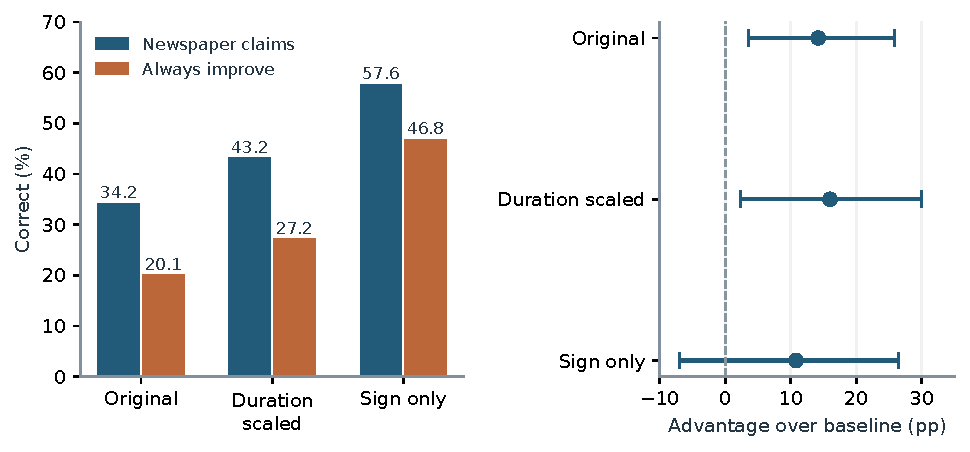
\includegraphics[width=\linewidth]{employment_sensitivity.pdf}
\caption{Higher measured accuracy does not imply a larger advantage over the comparator. Left: claim and baseline correctness under each rule. Right: paired baseline-relative differences with the saved 95\% five-year block intervals. Claims and weights are fixed across specifications.}\label{fig:employment}
\end{figure*}

The accuracy increase from 34.2\% to 57.6\% is 23.4 percentage points. Yet the fixed comparator improves by 26.8 points, so the newspaper advantage is smaller under sign-only scoring. The flat-band choice changes which outcomes are common: the always-flat comparator scores 50.6\% under the original rule, 35.2\% under duration scaling, and 5.8\% under sign-only scoring. Under the original band, newspapers underperform always-flat by 16.4 points even though they outperform always-improve. These facts show why reporting only one favorable baseline comparison is incomplete.

The results are descriptive specification sensitivity, not a test that the original band is logically invalid. A tolerance band can be appropriate for a forecast of economically material change. The source might instead commit to any increase, in which case sign-only scoring may be closer. Choosing the rule because it produces the highest hit rate would use outcomes to decide what the forecast meant. Source interpretation should precede that choice.

\subsection{Employment growth and unemployment are different targets}
Table~\ref{tab:target} reports the alternative-target exercise, which compares falling unemployment with rising payroll employment on the same 9,260 claims. After orienting both series toward improving labor-market conditions, sign-only outcomes disagree on 21.95\% of article-weighted observations. Employment can grow while the unemployment rate rises, for example if the labor force expands sufficiently. Benchmark disagreement is therefore not automatically a data error. It is evidence that the two economic questions are different.\evidence{M2}

\begin{table*}[t]
\caption{Changing the employment benchmark reverses the baseline-relative point estimate}\label{tab:target}
\centering\small
\begin{tabularx}{\linewidth}{Xrrrr}
\toprule
Sign-only outcome & Claims correct & Baseline & Gap (pp) & 95\% block interval\\
\midrule
Unemployment falls & 57.6\% & 46.8\% & +10.8 & [$-7.0$, 26.5]\\
Payroll employment rises & 55.1\% & 63.3\% & $-8.2$ & [$-33.2$, 19.0]\\
\bottomrule
\end{tabularx}
\note{Same 9,260 claims with common endpoint support and equal article weights. Both comparators always predict improving labor-market conditions, mapped to the relevant series. This is an alternative interpretation of broad employment labels, not a source-validated relabeling of every claim. The saved alternative-target exercise also preserves frozen-versus-refreshed-series checks. Source: M2.}
\end{table*}

The newspaper hit rate changes only modestly, from 57.6\% to 55.1\%, but the baseline rises from 46.8\% to 63.3\%. The resulting advantage changes by approximately $-19.0$ percentage points. The intervals are wide and include zero for both sign-only comparisons. The robust conclusion is the sensitivity of the point estimates and comparative interpretation, not established newspaper superiority under one target and inferiority under another.

This distinction extends beyond employment. Lower inflation is a decline in the rate of price growth, whereas falling prices are a decline in the price level. Slower output growth can coexist with rising output. A recession onset is an event, whereas an industrial-production endpoint change describes a particular series over a particular interval. An extractor that assigns only a broad topic cannot resolve these meanings by itself.

For fixed claims and weights, an elementary bound clarifies the arithmetic. If the same normalized prediction is scored against two outcome labelings, then
\begin{equation}
 |\widehat A_s-\widehat A_{s'}|
 \leq \frac{\sum_i w_i\mathbf{1}\{y_i^{(s)}\neq y_i^{(s')}\}}{\sum_i w_i}.
 \label{eq:bound}
\end{equation}
Only observations whose outcome labels change can change correctness. This follows directly from the indicator definition and is not offered as a novel theorem. It also does not establish which labeling is right. For a baseline-relative gap, both the claim and comparator terms can change; under the same fixed prediction mapping the analogous bound is twice the weighted disagreement. The empirical task remains identifying the economic proposition in the source.

\subsection{Dependence, uncertainty, and selection}
Claims are not independent economic trials. Multiple articles can discuss the same month, and overlapping horizons share much of the same outcome path. The primary historical sensitivity intervals therefore resample occupied five-year publication blocks in pairs, preserving model or rule comparisons within a block. Two- and ten-year versions are retained in the saved outputs. The employment analysis has 14 occupied five-year blocks; thousands of claims do not create thousands of independent business-cycle realizations.

These intervals condition on the saved observations, interpretations, and fitted outputs. They do not capture uncertainty about source validity, target choice, or the process that selected specifications after earlier results were inspected. The publication specification was written after historical analyses had been viewed. It is not a preregistration, and the sensitivity analyses do not create a fresh holdout. We consequently report their magnitudes and stability rather than promote a winning rule from observed performance.

\section{Predictive applications: historical and modern evidence}
\subsection{Predicting correctness of an extracted claim}
The first predictive task estimates $P(z_i^{(s)}=1\mid\mathcal I_i)$, where $z_i^{(s)}$ is the deterministic correctness label and $\mathcal I_i$ contains permitted information at publication. This is a forecast of claim correctness under the scoring contract. It is neither the probability that extraction is valid nor the probability of a recession.

The frozen recurrent model uses the previous twelve complete calendar months of national forecast distributions across four topics. Each topic contributes five normalized direction shares, log claim count, and an observed-coverage indicator. Current-claim inputs are topic, paper family, voice, hedging category, direction, horizon basis, and numeric horizon. The current publication month is excluded from the sequence. No quotation text, speaker identity, realized outcomes, prior hit rates, crisis annotations, verifier prose, NBER state, or macro reference value enters as a feature. Log counts describe export volume, not a normalized attention measure.\evidence{P2}

Table~\ref{tab:rnn} reports historical predictive performance. A one-layer, 24-unit gated recurrent unit (GRU) feeds a 32-unit head with 15\% dropout. Predictions average three preset seeds. Training publications precede 1985; validation spans 1985--1994; final historical evaluation spans 1995--2010. Outcomes are purged from earlier splits unless their endpoint plus a three-month allowance precedes the next split. After 7,743 purged claims, the split counts are 70,722 training, 39,536 validation, and 56,807 evaluation claims. Preprocessing is fitted on training data only; validation log loss selects epochs.

\begin{table*}[t]
\caption{Historical claim-correctness prediction, 1995--2010}\label{tab:rnn}
\centering\small
\begin{tabularx}{\linewidth}{Xrrrr}
\toprule
Model & AUC & Average precision & Brier & Log loss\\
\midrule
Training-prevalence constant & .500 & .409 & .244 & .681\\
Metadata logistic & .678 & .579 & .218 & .629\\
Metadata + history logistic & .634 & .596 & .236 & .692\\
Frozen GRU ensemble & .761 & .683 & .193 & .565\\
\bottomrule
\end{tabularx}
\note{Equal article weights; 56,807 claims. Correctness prevalence is .409. Binary Brier has range 0--1 and lower is better; AUC and average precision measure discrimination. These saved development comparisons do not establish a universally superior model. Source: P2.}
\end{table*}

The ensemble's average-precision advantage over the metadata-plus-history logistic control is 0.0876, with a saved five-year block interval of $[-0.1912,0.2102]$ based on four blocks and 400 draws. Separate saved block-swap tests of Brier differences also fail to establish superiority after the reported adjustment. The small number of time blocks sharply limits inferential resolution. Moreover, the logistic comparison does not isolate recurrence from nonlinear function approximation; a matched feed-forward neural control has not been supplied.

Although features respect publication ordering, outcome labels use frozen revised historical series. A three-month release allowance alone cannot prove that every revised value was known then. Modern language models used for historical extraction can also contain later knowledge in their pretrained parameters. Restricting the prompt to source text reduces overt hindsight use but does not certify its absence. This exercise is chronological prediction from reconstructed historical features, not a claim that the entire modern extraction system could have operated in 1900.

\subsection{Modern transfer of frozen claim models, 2011--2026}
On 56,886 mature, supported modern claims, the frozen baseline GRU achieves article-weighted AUC 0.738 and Brier loss 0.1770, compared with AUC 0.654 and Brier loss 0.1936 for the metadata-plus-history logistic control. The Brier improvement is 0.0165, with a paired five-year block interval of $[-0.0092,0.0376]$. Thus the point estimates favor the recurrent model, while the interval does not establish a stable improvement. The GRU with both political separation and forecast disagreement attains AUC 0.749, also without an established incremental Brier gain. No models are selected or recalibrated on these modern results.\evidence{N1}

Transfer is strongly topic-dependent: baseline-GRU AUC is 0.906 for prices, 0.788 for markets, 0.767 for general business, and 0.306 for employment. These outcomes concern correctness under the existing scoring contract, not the validity of extracted passages. Undocumented prior modern outcome exposure, calibration weaknesses, and the employment failure limit the generalization claim. Appendix~\ref{app:modern} summarizes the model comparison and calibration limits. None of these modern claims is pooled into the historical measurement-sensitivity estimates.

\subsection{Incremental information for aggregate production}
The second task predicts a six-month industrial-production direction from month $t-1$ to $t+5$, with an inclusive $\pm2\%$ flat band. Its unit is a monthly forecast origin. It compares a selected macro-only model with the same model augmented by four newspaper signals: recent net direction, common-paper change, disagreement, and cross-paper dispersion. A recent class-frequency comparator is retained.\evidence{P1}

The core evaluation covers 408 months from January 1977 through December 2010. Each January, training-only forward validation chooses among twelve combinations of macro feature set, regularization strength, and expanding versus recent-120-month estimation windows. Macro features are production growth alone or production growth plus unemployment change. Historical label vintages are used at inner and outer refits. The press-augmented regression inherits the macro-selected settings and training months; it is not retuned to maximize its evaluation gain. The procedure was nevertheless designed after inspection of an earlier historical comparator, so the reported period is not untouched.

Multiclass Brier loss is the sum of squared errors over fall, flat, and rise and ranges from zero to two. Macro-only Brier is 0.6327, compared with 0.6228 for macro plus press and 0.6443 for recent class frequencies. The primary improvement, macro-only minus macro-plus-press loss, is 0.0099. Its paired five-year block interval is $[-0.0637,0.0808]$, with seven calendar blocks. Log loss falls from 0.9989 to 0.9606, and accuracy rises from 35.8\% to 44.1\%; these descriptive gains do not remove uncertainty in the primary comparison.

When the already-inspected 2007--2009 scoring months are omitted, 372 months remain. Macro-only Brier is 0.6164 and macro-plus-press Brier is 0.6214, an improvement of $-0.0050$. This is a scoring exclusion using the saved forecasts, not a new fit and not evidence from excluded crisis-window exports. It shows that the average gain is sensitive to a particular evaluation episode. The manuscript therefore does not claim a stable incremental forecasting advantage across eras.

\section{Discussion}
The paired audit shows why candidate precision is an incomplete criterion for computational measurement. The additional verifier removes more human-rejected than human-accepted passages and increases inclusion precision in both review frames. Yet its survivors do not show a consistent increase in agreement on the annotations needed for economic analysis. Historical horizon agreement declines against both reviewers, and scope agreement remains around two-thirds. A filter that asks whether a passage is a forecast is not, by itself, a procedure for establishing what was forecast.

The economic sensitivity analysis shows the consequence of leaving that interpretation unresolved. On identical employment claims, changing an outcome band affects newspaper and comparator accuracy differently. Replacing the unemployment outcome with payroll employment changes the sign of the baseline-relative point estimate. This is evidence about the stability of the implemented measurement, not a causal claim about newspaper competence or a demonstration that one economic benchmark is universally preferable. The source proposition must determine which target is appropriate.

These findings suggest a practical allocation of validation effort. After inclusion screening, source review should focus on the quantity, geographic scope, conditionality, and endpoint that define the intended economic estimand. Human agreement should be reported separately for those fields, and sensitivity analysis should hold claims and weights fixed when comparing outcome mappings. The audit's rejected and retained records, including unresolved cases, must remain traceable. Additional filtering should be evaluated for both removed false positives and lost accepted claims.

Several limitations constrain generalization. Retrieval coverage and incomplete processing denominators limit representativeness. The positive-candidate sample leaves full-document recall unknown. The two reviewers disagree on some claims and were not both fully blind to all study information; no adjudication resolves that uncertainty. The additional pass is a single realization on production survivors, with one parsing failure retained. No population-weighted or statistically significant filtering gain is asserted. Revised outcomes, pretrained language models, and prior inspection of evaluation periods limit historical real-time and confirmatory interpretations. Few calendar blocks and overlapping forecast windows limit effective information for predictive comparisons.

A stronger subsequent design would sample complete documents, including documents with no forecasts, and obtain source interpretations before inspecting outcomes. It would compare extraction and verification configurations on common documents and freeze economic targets and evaluation rules before a new period matures. The current evidence already supports a narrower conclusion: inexpensive candidate generation can make historical expectations accessible, but inclusion filtering, annotation validation, and economic scoring require separate empirical checks.

\section{Conclusion}
This study links two-reviewer source validation, a single additional verification pass, and matched economic scoring in a large newspaper-forecast application. Additional filtering improves inclusion precision while losing some human-accepted claims; it leaves specific-label agreement largely unchanged or slightly worse. The historical employment exercise further shows that alternative outcome definitions can reverse comparative point estimates on the same observations. The modern extension adds separate evidence on validation and transfer, without establishing stable predictive superiority. These results support treating candidate validity, source interpretation, and economic correctness as distinct measurement claims, each requiring its own evidence.

\section*{Statements and Declarations}
\subsection*{Data and code availability}
The analysis code, source-linked categorical review labels, frozen additional-pass decisions, and derived results are held in the project repository. Appendix~\ref{app:evidence} identifies the saved evidence and reproduction instructions; the 300-record additional-pass package is committed at \texttt{794bacc}. A permanent public archive identifier or reviewer-access URL must be supplied by the authors before submission. ProQuest article text and quotations are not redistributed here. Source-level replication requires authorized access to the relevant ProQuest newspaper holdings and TDM Studio; source addresses and checksums support matching within that environment. This statement does not grant rights to third-party content.

\subsection*{Use of artificial intelligence}
GPT-4o mini supplied automated extraction labels and the additional verification decisions; its role, parameters, and limitations are described in the methods. AI assistance supported code, analysis, and manuscript drafting and revision. Human source annotations are preserved separately. No language model is an author; responsibility for the submitted analysis and wording remains with the human authors.

\subsection*{Funding, competing interests, and author contributions}
Author confirmation is pending for funding, financial and non-financial competing interests, affiliation details and individual contributions. These declarations must be completed by the authors; absence of information is not represented as absence of funding or interests.

\subsection*{Ethics and consent}
The study analyzes published newspaper material and source annotations. The authors must confirm the applicable institutional ethics determination and whether any review-participant consent requirement applies before submission. No approval or exemption is inferred from the existing repository.

\FloatBarrier
\appendix
\section{Modern model comparison}\label{app:modern}
The separate modern evaluation uses frozen historical parameters and 56,886 mature, supported claims. Table~\ref{tab:modern} retains all saved model arms. Results use the October 20, 2026 snapshots, including production, CPI, and unemployment through June 2026, with a three-month maturity allowance and no interpolation. Prior outcome exposure is undocumented; this is an exploratory extension.\evidence{N1}

\begin{table*}[t]
\caption{Modern claim-correctness prediction: frozen baseline and secondary arms}\label{tab:modern}
\centering\small
\begin{tabularx}{\linewidth}{Xrrrr}
\toprule
Model & AUC & Brier & Log loss & Accuracy\\
\midrule
Metadata logistic & .662 & .1983 & .5861 & .6987\\
Metadata + history logistic & .654 & .1936 & .5789 & .7223\\
Frozen GRU, baseline & .738 & .1770 & .5347 & .7539\\
GRU + political separation & .692 & .1826 & .5503 & .7618\\
GRU + forecast disagreement & .712 & .1819 & .5479 & .7388\\
GRU + both measures & .749 & .1742 & .5259 & .7610\\
Historical 8-unit challenger & .723 & .1775 & .5792 & .7743\\
\bottomrule
\end{tabularx}
\note{56,886 common claims, equal article weights. Positive correctness prevalence is .2868. The historical challenger is disclosed without promotion. Accuracy uses a .5 decision threshold; a classifier always predicting incorrect would attain .7132 accuracy from the evaluated prevalence, so accuracy alone is not a strong skill diagnostic. Source: N1.}
\end{table*}

The primary GRU's Brier improvement over metadata-plus-history logistic is 0.0165, with a paired five-year block interval of $[-0.0092,0.0376]$. Adding both measures improves Brier by 0.0028, with interval $[-0.0058,0.0191]$. Four blocks contain 17,784, 18,017, 21,072, and 13 claims, limiting temporal replication. Political separation uses prior House rollcall differences; forecast disagreement measures opposing business-forecast directions. Both are lagged, and neither identifies a causal political effect. Definitions and coverage rules are preserved in P3.

Calibration is weak: in the .8--.9 bin, predicted correctness averages .853 versus observed .619 (2,168 claims); in the highest bin, .912 versus .743 (474 claims). Employment AUC of .306 concerns the model's ranking of correctness, not the forecasts' hit rate. No modern recalibration or post hoc reversal is applied. Full subgroup metrics and secondary analyses remain in the repository.

\section{Additional label validation}\label{app:labels}
Table~\ref{tab:modernfields} reports all eleven modern fields. These sample agreements are conditional on each reviewer's inclusion, not population estimates or extraction recall. Filtering changes the evaluated subset without changing the original annotations.

\begin{table*}[t]
\caption{Modern machine--human label agreement before and after filtering}\label{tab:modernfields}
\centering\small
\begin{tabularx}{\linewidth}{Xrrrr}
\toprule
& \multicolumn{2}{c}{Reviewer 1} & \multicolumn{2}{c}{Reviewer 2}\\
Field & Before & After & Before & After\\
\midrule
Topic & 29/35 (82.9\%) & 26/32 (81.2\%) & 29/33 (87.9\%) & 27/31 (87.1\%)\\
Direction & 29/35 (82.9\%) & 26/32 (81.2\%) & 30/33 (90.9\%) & 28/31 (90.3\%)\\
Price direction & 30/35 (85.7\%) & 27/32 (84.4\%) & 28/33 (84.8\%) & 26/31 (83.9\%)\\
Unemployment direction & 31/35 (88.6\%) & 28/32 (87.5\%) & 28/33 (84.8\%) & 26/31 (83.9\%)\\
Horizon (months) & 26/35 (74.3\%) & 24/32 (75.0\%) & 27/33 (81.8\%) & 25/31 (80.6\%)\\
Confidence & 22/35 (62.9\%) & 20/32 (62.5\%) & 23/33 (69.7\%) & 22/31 (71.0\%)\\
Voice & 24/35 (68.6\%) & 22/32 (68.8\%) & 22/33 (66.7\%) & 20/31 (64.5\%)\\
Speaker name & 27/35 (77.1\%) & 26/32 (81.2\%) & 21/33 (63.6\%) & 21/31 (67.7\%)\\
Scope & 24/35 (68.6\%) & 22/32 (68.8\%) & 23/33 (69.7\%) & 22/31 (71.0\%)\\
Quoted forecaster & 23/35 (65.7\%) & 21/32 (65.6\%) & 23/33 (69.7\%) & 22/31 (71.0\%)\\
Current state & 27/35 (77.1\%) & 24/32 (75.0\%) & 27/33 (81.8\%) & 25/31 (80.6\%)\\
\bottomrule
\end{tabularx}
\note{Exact agreement on each reviewer\textquotesingle s included claims. Different before/after denominators reflect filtering, not relabeling. NA matches are included; missing/uncertain fields receive no match credit. Source: V5.}
\end{table*}

Among claims accepted by both reviewers, human--human direction agreement is 150/166 (90.4\%) historically and 27/30 (90.0\%) in the modern sample; horizon agreement is 147/166 (88.6\%) and 26/30 (86.7\%). Speaker-name agreement is lower, at 128/166 (77.1\%) and 20/30 (66.7\%). Full field comparisons, category-specific precision and recall, confusion counts, and missing-label counts are preserved in V4--V5. Their denominators differ from machine--human agreement.

\section{Evidence and reproduction}\label{app:evidence}
Evidence identifiers refer to saved files below, relative to \pathcode{data/scored/proquest/}. Source exports and human labels remain unchanged. Review status follows the human attestations through October 22, 2026; it does not certify every corpus claim.

\begingroup\raggedright
\begin{description}[style=nextline,font=\bfseries,leftmargin=0pt,labelwidth=0pt,labelsep=0pt]
\item[H1--H2: Corpus and scoring.]
\pathcode{inventory.json}; \pathcode{descriptive/summary.json}; \pathcode{publication/evidence.json}.
\item[V1--V3: Human reviews and provenance.]
\pathcode{source_review_150_v1/human_reconciliation_summary.json}; \pathcode{source_review_additional150_v1/summary.json}; \pathcode{reviewer2_300_v1/manifest.json}, with the respective frozen labels, protocols, and attestations.
\item[V4--V5: Paired comparisons and additional pass.]
\pathcode{verification_pass_audit_20261022/summary.json}; \pathcode{reverify300_20261022/summary.json}, with paired records, imported decisions, input hashes, and the import receipt.
\item[M1--M2: Matched employment comparisons.]
\pathcode{benchmark_interpretation_v2/primary_comparisons.csv}; \pathcode{alternative_targets_v1/primary_comparisons.csv}, with their specifications. Use verified, machine-stated, non-NBER employment claims and saved five-year blocks.
\item[P1--P3: Historical prediction and feature definitions.]
\pathcode{macro_benchmark/evaluation_spec.json}; \pathcode{rnn/summary.json}; \pathcode{rnn_permutation/paired_tests.csv}; \pathcode{polarization/evaluation_spec.json}.
\item[N1: Modern evaluation.]
\pathcode{modern_analysis_v1/claim_summary.json}; \pathcode{modern_analysis_v1/claim_paired_intervals.json}, with metrics, subgroup, and calibration files in the same directory.
\end{description}
\endgroup

From the repository root, \pathcode{scripts/build_jcss_package.py} generates the journal source package from saved results; compile its \texttt{main.tex} with pdfLaTeX until references settle. Broader analysis instructions are in \pathcode{docs/PROQUEST_REPRODUCIBILITY.md}. Source-level replication requires authorized ProQuest access. The build receipt in \pathcode{data/scored/proquest/paper_jcss_v1/} records artifact hashes and checks.

\FloatBarrier
\begingroup
\small
\setlength{\bibsep}{5pt}
\begin{thebibliography}{99}
\bibitem[Mathy and Stekler(2017)]{mathy2017}
Mathy, G., and Stekler, H. (2017).
Expectations and forecasting during the Great Depression: Real-time evidence from the business press.
\textit{Journal of Macroeconomics}, 53, 1--15.
\url{https://doi.org/10.1016/j.jmacro.2017.05.006}.

\bibitem[Gentzkow et~al.(2019)]{gentzkow2019}
Gentzkow, M., Kelly, B., and Taddy, M. (2019).
Text as data. \textit{Journal of Economic Literature}, 57(3), 535--574.
\url{https://doi.org/10.1257/jel.20181020}.

\bibitem[Bybee et~al.(2024)]{bybee2024}
Bybee, L., Kelly, B., Manela, A., and Xiu, D. (2024).
Business news and business cycles. \textit{The Journal of Finance}, 79(5), 3105--3147.
\url{https://doi.org/10.1111/jofi.13377}.

\bibitem[Barbaglia et~al.(2023)]{barbaglia2022}
Barbaglia, L., Consoli, S., and Manzan, S. (2023). Forecasting with economic news. \textit{Journal of Business \& Economic Statistics}, 41(3), 708--719.
\url{https://doi.org/10.1080/07350015.2022.2060988}.

\bibitem[Tetlock(2007)]{tetlock2007}
Tetlock, P. C. (2007). Giving content to investor sentiment: The role of media in the stock market. \textit{The Journal of Finance}, 62(3), 1139--1168.
\url{https://doi.org/10.1111/j.1540-6261.2007.01232.x}.
\bibitem[Garc\'{i}a(2013)]{garcia2013}
Garc\'{i}a, D. (2013). Sentiment during recessions. \textit{The Journal of Finance}, 68(3), 1267--1300.
\url{https://doi.org/10.1111/jofi.12027}.

\bibitem[Baker et~al.(2016)]{baker2016}
Baker, S. R., Bloom, N., and Davis, S. J. (2016). Measuring economic policy uncertainty. \textit{The Quarterly Journal of Economics}, 131(4), 1593--1636.
\url{https://doi.org/10.1093/qje/qjw024}.

\bibitem[Baker et~al.(n.d.)]{bakerhistorical}
Baker, S. R., Bloom, N., and Davis, S. J. (n.d.). \textit{US historical economic policy uncertainty index} [Data set]. Economic Policy Uncertainty. Retrieved August 3, 2026, from
\url{https://www.policyuncertainty.com/us_historical.html}.

\bibitem[FRB Philadelphia(n.d.-b)]{philalivingston}
Federal Reserve Bank of Philadelphia. (n.d.-b). \textit{Livingston Survey} [Data set]. Real-Time Data Research Center. Retrieved August 3, 2026, from
\url{https://www.philadelphiafed.org/surveys-and-data/real-time-data-research/livingston-survey}.

\bibitem[FRB Philadelphia(n.d.-c)]{philaspf}
Federal Reserve Bank of Philadelphia. (n.d.-c). \textit{Survey of Professional Forecasters} [Data set]. Real-Time Data Research Center. Retrieved August 3, 2026, from
\url{https://www.philadelphiafed.org/surveys-and-data/real-time-data-research/survey-of-professional-forecasters}.

\bibitem[FRB Philadelphia(n.d.-a)]{philagreenbook}
Federal Reserve Bank of Philadelphia. (n.d.-a). \textit{Tealbook (formerly Greenbook) data sets} [Data set]. Real-Time Data Research Center. Retrieved August 3, 2026, from
\url{https://www.philadelphiafed.org/surveys-and-data/real-time-data-research/greenbook}.

\bibitem[Campbell and Moore(2024)]{campbell2024}
Campbell, S., and Moore, D. A. (2024). Overprecision in the Survey of Professional Forecasters. \textit{Collabra: Psychology}, 10(1), Article 92953.
\url{https://doi.org/10.1525/collabra.92953}.

\bibitem[Shapiro et~al.(2022)]{shapiro2020}
Shapiro, A. H., Sudhof, M., and Wilson, D. J. (2022). Measuring news sentiment. \textit{Journal of Econometrics}, 228(2), 221--243.
\url{https://doi.org/10.1016/j.jeconom.2020.07.053}.

\bibitem[Grimmer and Stewart(2013)]{grimmer2013}
Grimmer, J., and Stewart, B. M. (2013).
Text as data: The promise and pitfalls of automatic content analysis methods for political texts.
\textit{Political Analysis}, 21(3), 267--297.
\url{https://doi.org/10.1093/pan/mps028}.

\bibitem[Loughran and McDonald(2011)]{loughran2011}
Loughran, T., and McDonald, B. (2011). When is a liability not a liability? Textual analysis, dictionaries, and 10-Ks. \textit{The Journal of Finance}, 66(1), 35--65.
\url{https://doi.org/10.1111/j.1540-6261.2010.01625.x}.

\bibitem[Gilardi et~al.(2023)]{gilardi2023}
Gilardi, F., Alizadeh, M., and Kubli, M. (2023).
ChatGPT outperforms crowd workers for text-annotation tasks.
\textit{Proceedings of the National Academy of Sciences}, 120(30), e2305016120.
\url{https://doi.org/10.1073/pnas.2305016120}.

\bibitem[Gneiting and Raftery(2007)]{gneiting2007}
Gneiting, T., and Raftery, A. E. (2007). Strictly proper scoring rules, prediction, and estimation. \textit{Journal of the American Statistical Association}, 102(477), 359--378.
\url{https://doi.org/10.1198/016214506000001437}.

\bibitem[Croushore and Stark(2001)]{croushore1999}
Croushore, D., and Stark, T. (2001). A real-time data set for macroeconomists. \textit{Journal of Econometrics}, 105(1), 111--130.
\url{https://doi.org/10.1016/S0304-4076(01)00072-0}.

\bibitem[Cawley and Talbot(2010)]{cawley2010}
Cawley, G. C., and Talbot, N. L. C. (2010). On over-fitting in model selection and subsequent selection bias in performance evaluation. \textit{Journal of Machine Learning Research}, 11, 2079--2107.
\url{https://www.jmlr.org/papers/v11/cawley10a.html}.

\bibitem[ProQuest(n.d.-a)]{proquesthistorical}
ProQuest. (n.d.-a). \textit{ProQuest Historical Newspapers} [Database]. Retrieved October 21, 2026, from
\url{https://about.proquest.com/en/products-services/pq-hist-news/}.

\bibitem[ProQuest(n.d.-b)]{proquesttdm}
ProQuest. (n.d.-b). \textit{TDM Studio} [Research platform]. Retrieved October 21, 2026, from
\url{https://about.proquest.com/en/products-services/TDM-Studio/}.

\bibitem[OpenAI(2024)]{openai4omini}
OpenAI. (2024). \textit{GPT-4o mini} [Large language model]. Model documentation; lists the gpt-4o-mini-2024-07-18 snapshot. Retrieved October 21, 2026, from
\url{https://developers.openai.com/api/docs/models/gpt-4o-mini}.

\bibitem[FRB St.\ Louis(n.d.-d)]{fredindpro}
Federal Reserve Bank of St.\ Louis. (n.d.-d). \textit{Industrial production: Total index} (INDPRO) [Data set]. FRED. Retrieved August 3, 2026, from
\url{https://fred.stlouisfed.org/series/INDPRO}.

\bibitem[FRB St.\ Louis(n.d.-b)]{fredcpi}
Federal Reserve Bank of St.\ Louis. (n.d.-b). \textit{Consumer Price Index for all urban consumers: All items in U.S. city average} (CPIAUCNS) [Data set]. FRED. Retrieved August 3, 2026, from
\url{https://fred.stlouisfed.org/series/CPIAUCNS}.

\bibitem[FRB St.\ Louis(n.d.-h)]{fredunrate}
Federal Reserve Bank of St.\ Louis. (n.d.-h). \textit{Unemployment rate} (UNRATE) [Data set]. FRED. Retrieved August 3, 2026, from
\url{https://fred.stlouisfed.org/series/UNRATE}.

\bibitem[Shiller(n.d.)]{shiller}
Shiller, R. J. (n.d.). \textit{Online data: Stock market data} [Data set]. Monthly stock-price, dividend, earnings, and interest-rate series. Retrieved October 21, 2026, from
\url{https://shillerdata.com/}.

\bibitem[FRB St.\ Louis(n.d.-a)]{fredpayems}
Federal Reserve Bank of St.\ Louis. (n.d.-a). \textit{All employees, total nonfarm} (PAYEMS) [Data set]. FRED. Retrieved October 21, 2026, from
\url{https://fred.stlouisfed.org/series/PAYEMS}.

\bibitem[FRB St.\ Louis(n.d.-f)]{fredusrec}
Federal Reserve Bank of St.\ Louis. (n.d.-f). \textit{NBER based recession indicators for the United States from the period following the peak through the trough} (USREC) [Data set]. FRED. Retrieved August 3, 2026, from
\url{https://fred.stlouisfed.org/series/USREC}.

\bibitem[NBER(n.d.)]{nber}
National Bureau of Economic Research. (n.d.). \textit{US business cycle expansions and contractions}. Retrieved August 3, 2026, from
\url{https://www.nber.org/research/business-cycle-dating}.

\end{thebibliography}
\endgroup
\end{document}
